% ============================================================
% Detection and Simulation of GPS Spoofing in Mobile Robots Using Sensor Cross-Validation — Thesis Defence
% Clean white theme, professional layout
% ============================================================
\documentclass[11pt]{beamer}

\usetheme{default}
\usecolortheme{seahorse}
\setbeamertemplate{navigation symbols}{}
\setbeamertemplate{footline}[frame number]
\setbeamertemplate{itemize items}[circle]
\setbeamerfont{title}{size=\Large}
\setbeamerfont{frametitle}{size=\large}
\setbeamerfont{itemize/enumerate body}{size=\small}
\setbeamerfont{itemize/enumerate subbody}{size=\footnotesize}
\setbeamercolor{title}{fg=blue!60!black}
\setbeamercolor{frametitle}{fg=blue!60!black,bg=blue!3}
\setbeamercolor{block title}{fg=white,bg=blue!60}
\setbeamercolor{block body}{bg=blue!5}
\setbeamercolor{item}{fg=blue!60}

\usepackage{graphicx}
\graphicspath{{figures/}}
\usepackage{booktabs}
\usepackage{tikz}
\usetikzlibrary{positioning}
\usepackage{amsmath}
\usepackage{hyperref}
\hypersetup{colorlinks=true,urlcolor=blue!60!black}

\title[Detection \& Simulation of GPS Spoofing]{Detection and Simulation of GPS Spoofing in Mobile Robots Using Sensor Cross-Validation}
\subtitle{SIT746 Research Project — Thesis Defence}
\author{Nikhil Sarwara \\[1mm] \tiny Student ID: 224234862 \quad|\quad Supervisor: Dr. Ananda Maiti}
\date{Trimester 1 2026}

\begin{document}

% ===================================================================
\begin{frame}
\maketitle
\vspace{-5mm}
\begin{center}
\tiny Deakin University — Faculty of Science, Engineering and Built Environment
\end{center}
\end{frame}

% ===================================================================
\begin{frame}{Outline}
\tableofcontents[hideallsubsections,sectionstyle=show,subsectionstyle=hide]
\end{frame}

% ===================================================================
\section{Introduction}
\begin{frame}{The GPS Spoofing Threat}
\begin{columns}[T]
\column{.55\textwidth}
\begin{itemize}\footnotesize
    \item GPS spoofing: counterfeit signals with false coordinates
    \item \textbf{Jamming} = denial; \textbf{Spoofing} = corruption of service
    \item PX4 EKF2 relies heavily on GPS for state estimation
    \item Spoofed signals report healthy fix — attack is silent
    \item Low-cost SDRs $\approx$\$300 make spoofing accessible
\end{itemize}
\vspace{2mm}
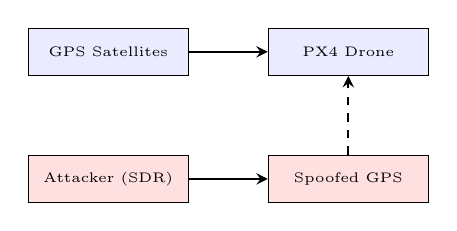
\begin{tikzpicture}[node distance=1cm,
    block/.style={rectangle,draw,fill=blue!8,text width=1.8cm,text centered,minimum height=.6cm,font=\tiny},
    red/.style={rectangle,draw,fill=red!12,text width=1.8cm,text centered,minimum height=.6cm,font=\tiny},
    arrow/.style={->,>=stealth,thick,font=\tiny}]
    \node[block] (s) {GPS Satellites};
    \node[block,right=of s] (d) {PX4 Drone};
    \node[red,below=of s] (a) {Attacker (SDR)};
    \node[red,right=of a] (f) {Spoofed GPS};
    \draw[arrow] (s) -- (d);
    \draw[arrow] (a) -- (f);
    \draw[arrow,dashed,red] (f.north) -- (d.south);
\end{tikzpicture}
\column{.45\textwidth}
\textbf{\footnotesize Real-World Incidents}
\begin{itemize}\footnotesize
    \item UT Austin 2012 — full 3D UAV control via spoofing\textsuperscript{[1]}
    \item Iran 2011 — GPS spoofing capture of RQ-170 Sentinel drone\textsuperscript{[2]}
    \item Commercial drone market projected \$54.6B by 2030\textsuperscript{[3]}
\end{itemize}
\vspace{1mm}
{\tiny
\textcolor{gray!70!black}{[1] Shepard et al., \textit{GPS World}, 2012: gpsworld.com/drone-hack} \\
\textcolor{gray!70!black}{[2] The Aviationist, 2011: theaviationist.com/2011/12/15/gps-spoofing} \\
\textcolor{gray!70!black}{[3] Grand View Research: grandviewresearch.com/press-release/commercial-drone-market}
}

\end{columns}
\end{frame}

% ===================================================================
\begin{frame}{Research Questions}
\begin{block}{RQ1: GPS Vulnerabilities}
\small What are the primary vulnerabilities of GPS in autonomous mobile robots to spoofing attacks?
\end{block}
\begin{block}{RQ2: Sensor Fusion for Real-Time Detection}
\small How can sensor fusion techniques effectively detect GPS spoofing in real time?
\end{block}
\begin{block}{RQ3: GPS Trust Index}
\small How can a dynamic GPS Trust Index be designed to quantify the reliability of GPS data?
\end{block}
\end{frame}

% ===================================================================
\section{System Architecture}
\begin{frame}{Simulation Environment \& Data Pipeline}
\begin{columns}[T]
\column{.48\textwidth}
\textbf{\scriptsize PX4 SITL + Gazebo}
\begin{itemize}\scriptsize
    \item Iris x500 quadcopter (3 kg)
    \item MAVLink telemetry @ 10 Hz
    \item 8 experimental + 60 synthetic flights
    \item 6 GPS spoofing attack modes
\end{itemize}
\vspace{1mm}
\textbf{\scriptsize 5-Stage ML Pipeline}
\begin{enumerate}\scriptsize
    \item Clean — filter, normalize, remove gaps
    \item Label — 8 physics-based heuristics
    \item Window — 30 samples, 50\% overlap
    \item Split — 70/15/15 train/val/test
    \item Train — Random Forest
\end{enumerate}
\column{.52\textwidth}
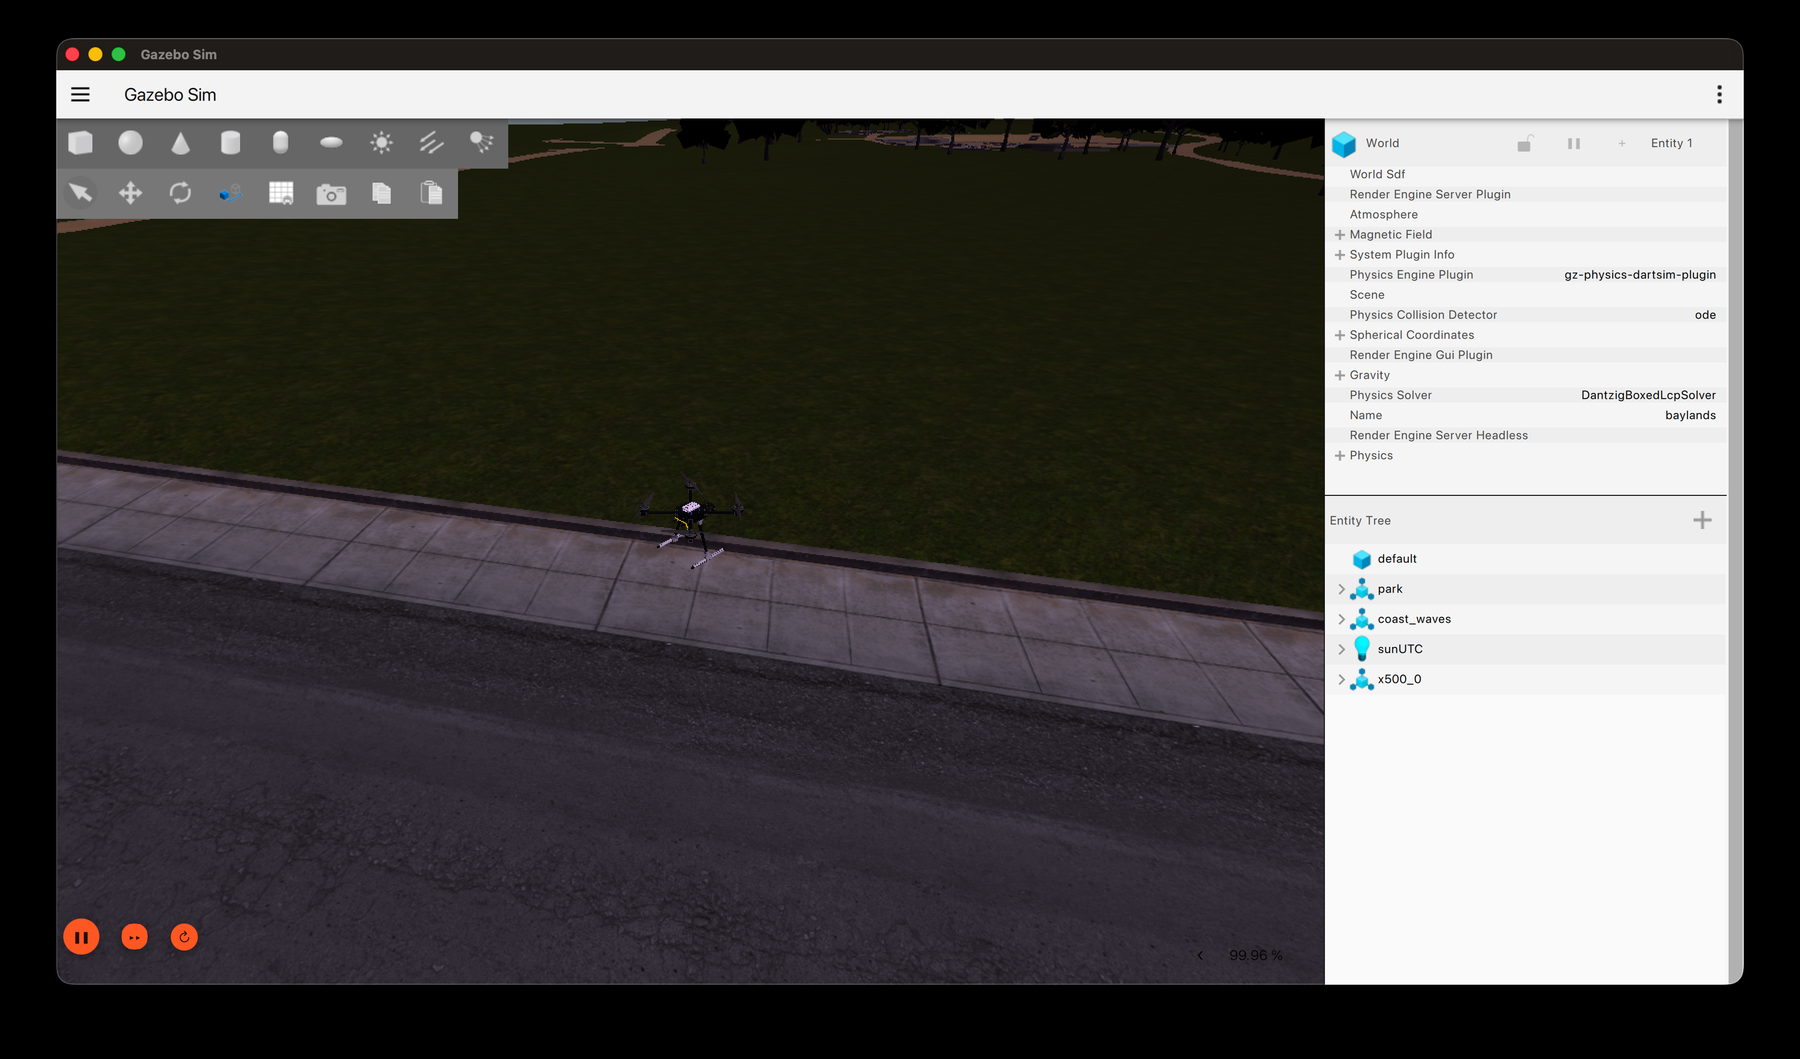
\includegraphics[width=\textwidth,height=.38\textheight,keepaspectratio]{px4_simulation_gazebo.png}
\vspace{1mm}
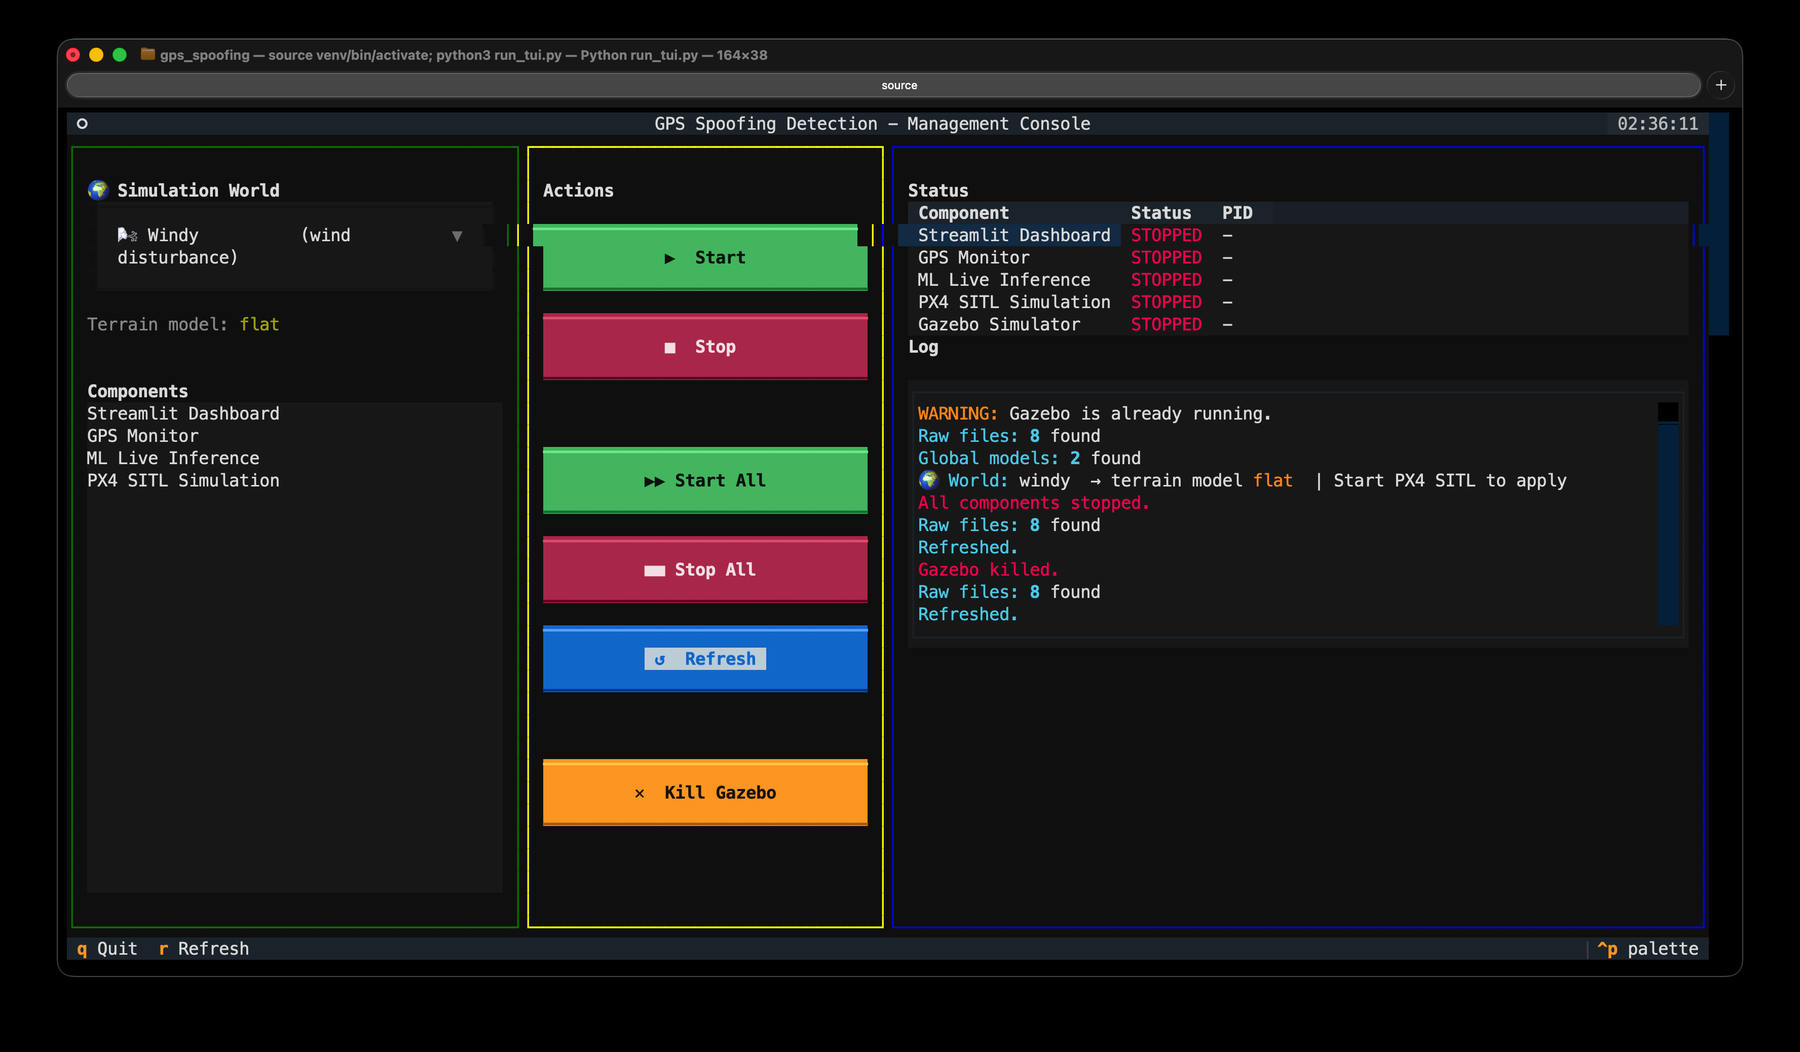
\includegraphics[width=\textwidth,height=.38\textheight,keepaspectratio]{tui_main.png}
\end{columns}
\end{frame}

% ===================================================================
\begin{frame}{GPS Spoofing Attack Injection}
\begin{columns}[T]
\column{.5\textwidth}
\textbf{\small Attack Mechanism}
\begin{itemize}\small
    \item MAVLink \texttt{GPS\_INPUT} messages @ 10 Hz
    \item \texttt{sysid=1, compid=220} (GPS source)
    \item Injected on UDP port 14580
    \item 6 modes: Drift, Ramp, Jump+Drift, Static, Teleport, Noise
\end{itemize}
\column{.5\textwidth}
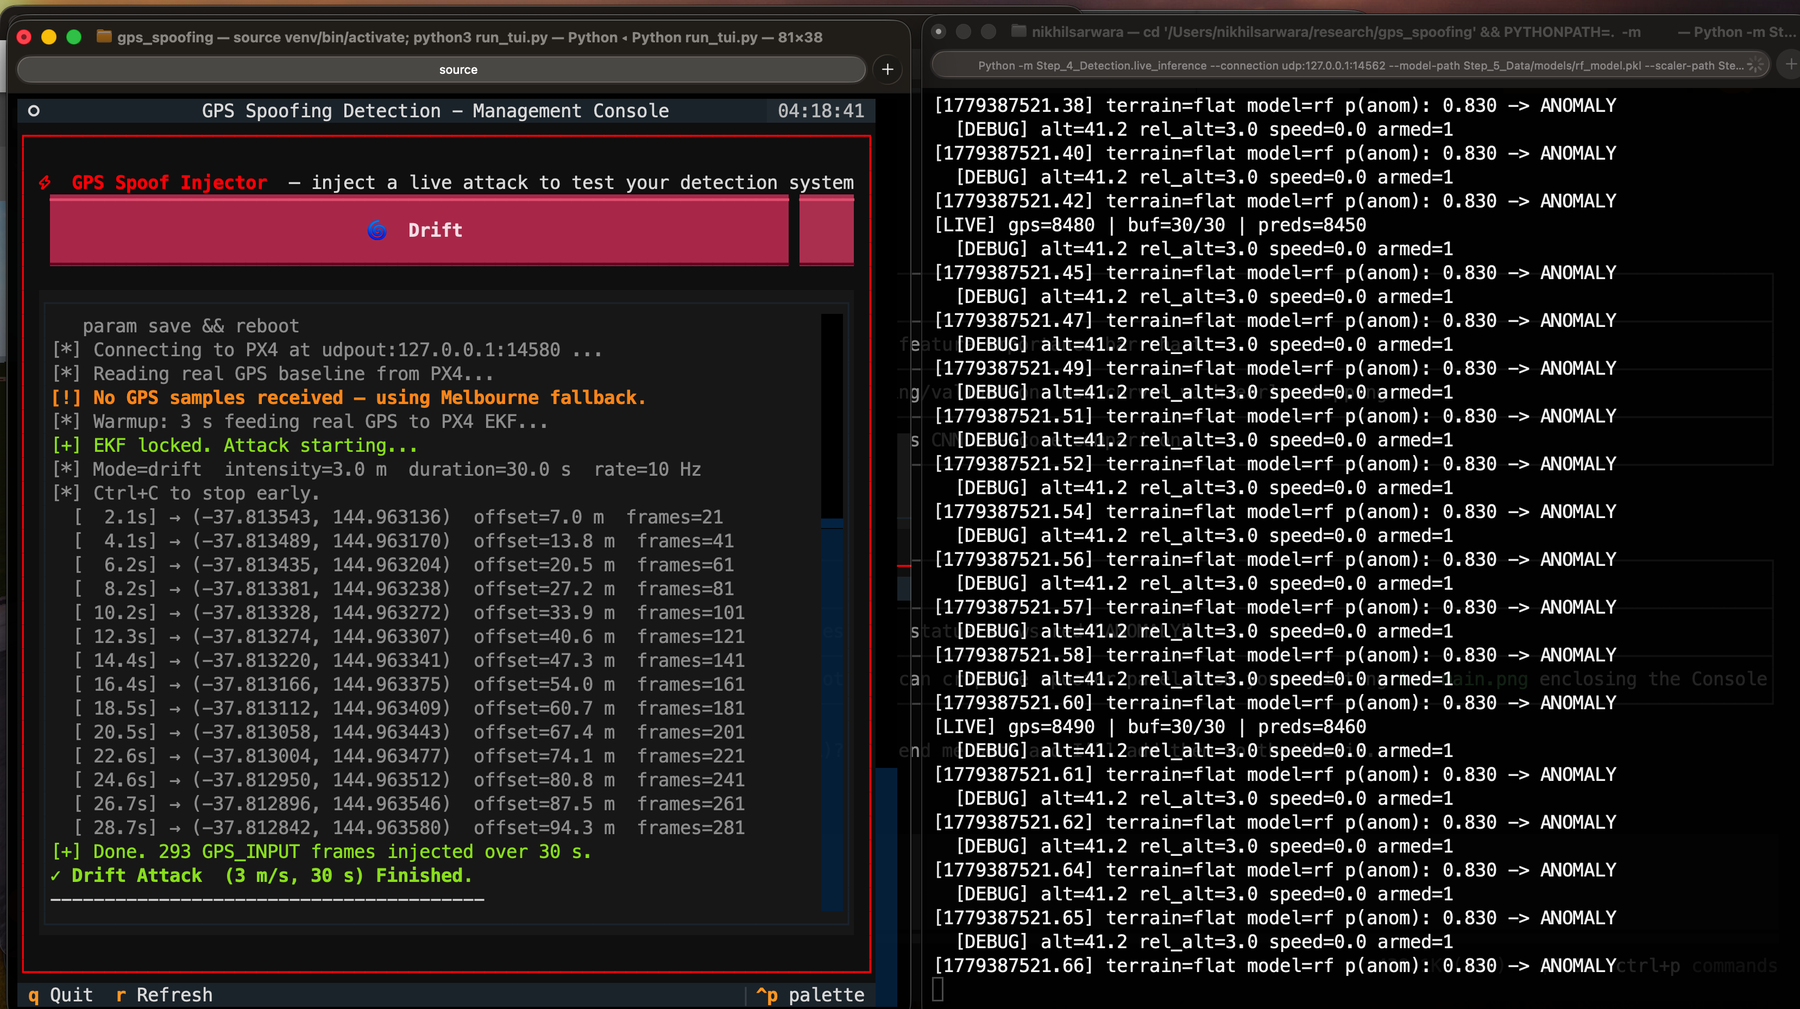
\includegraphics[width=\textwidth,height=.38\textheight,keepaspectratio]{gps_spoofer_output.png}
\vspace{1mm}
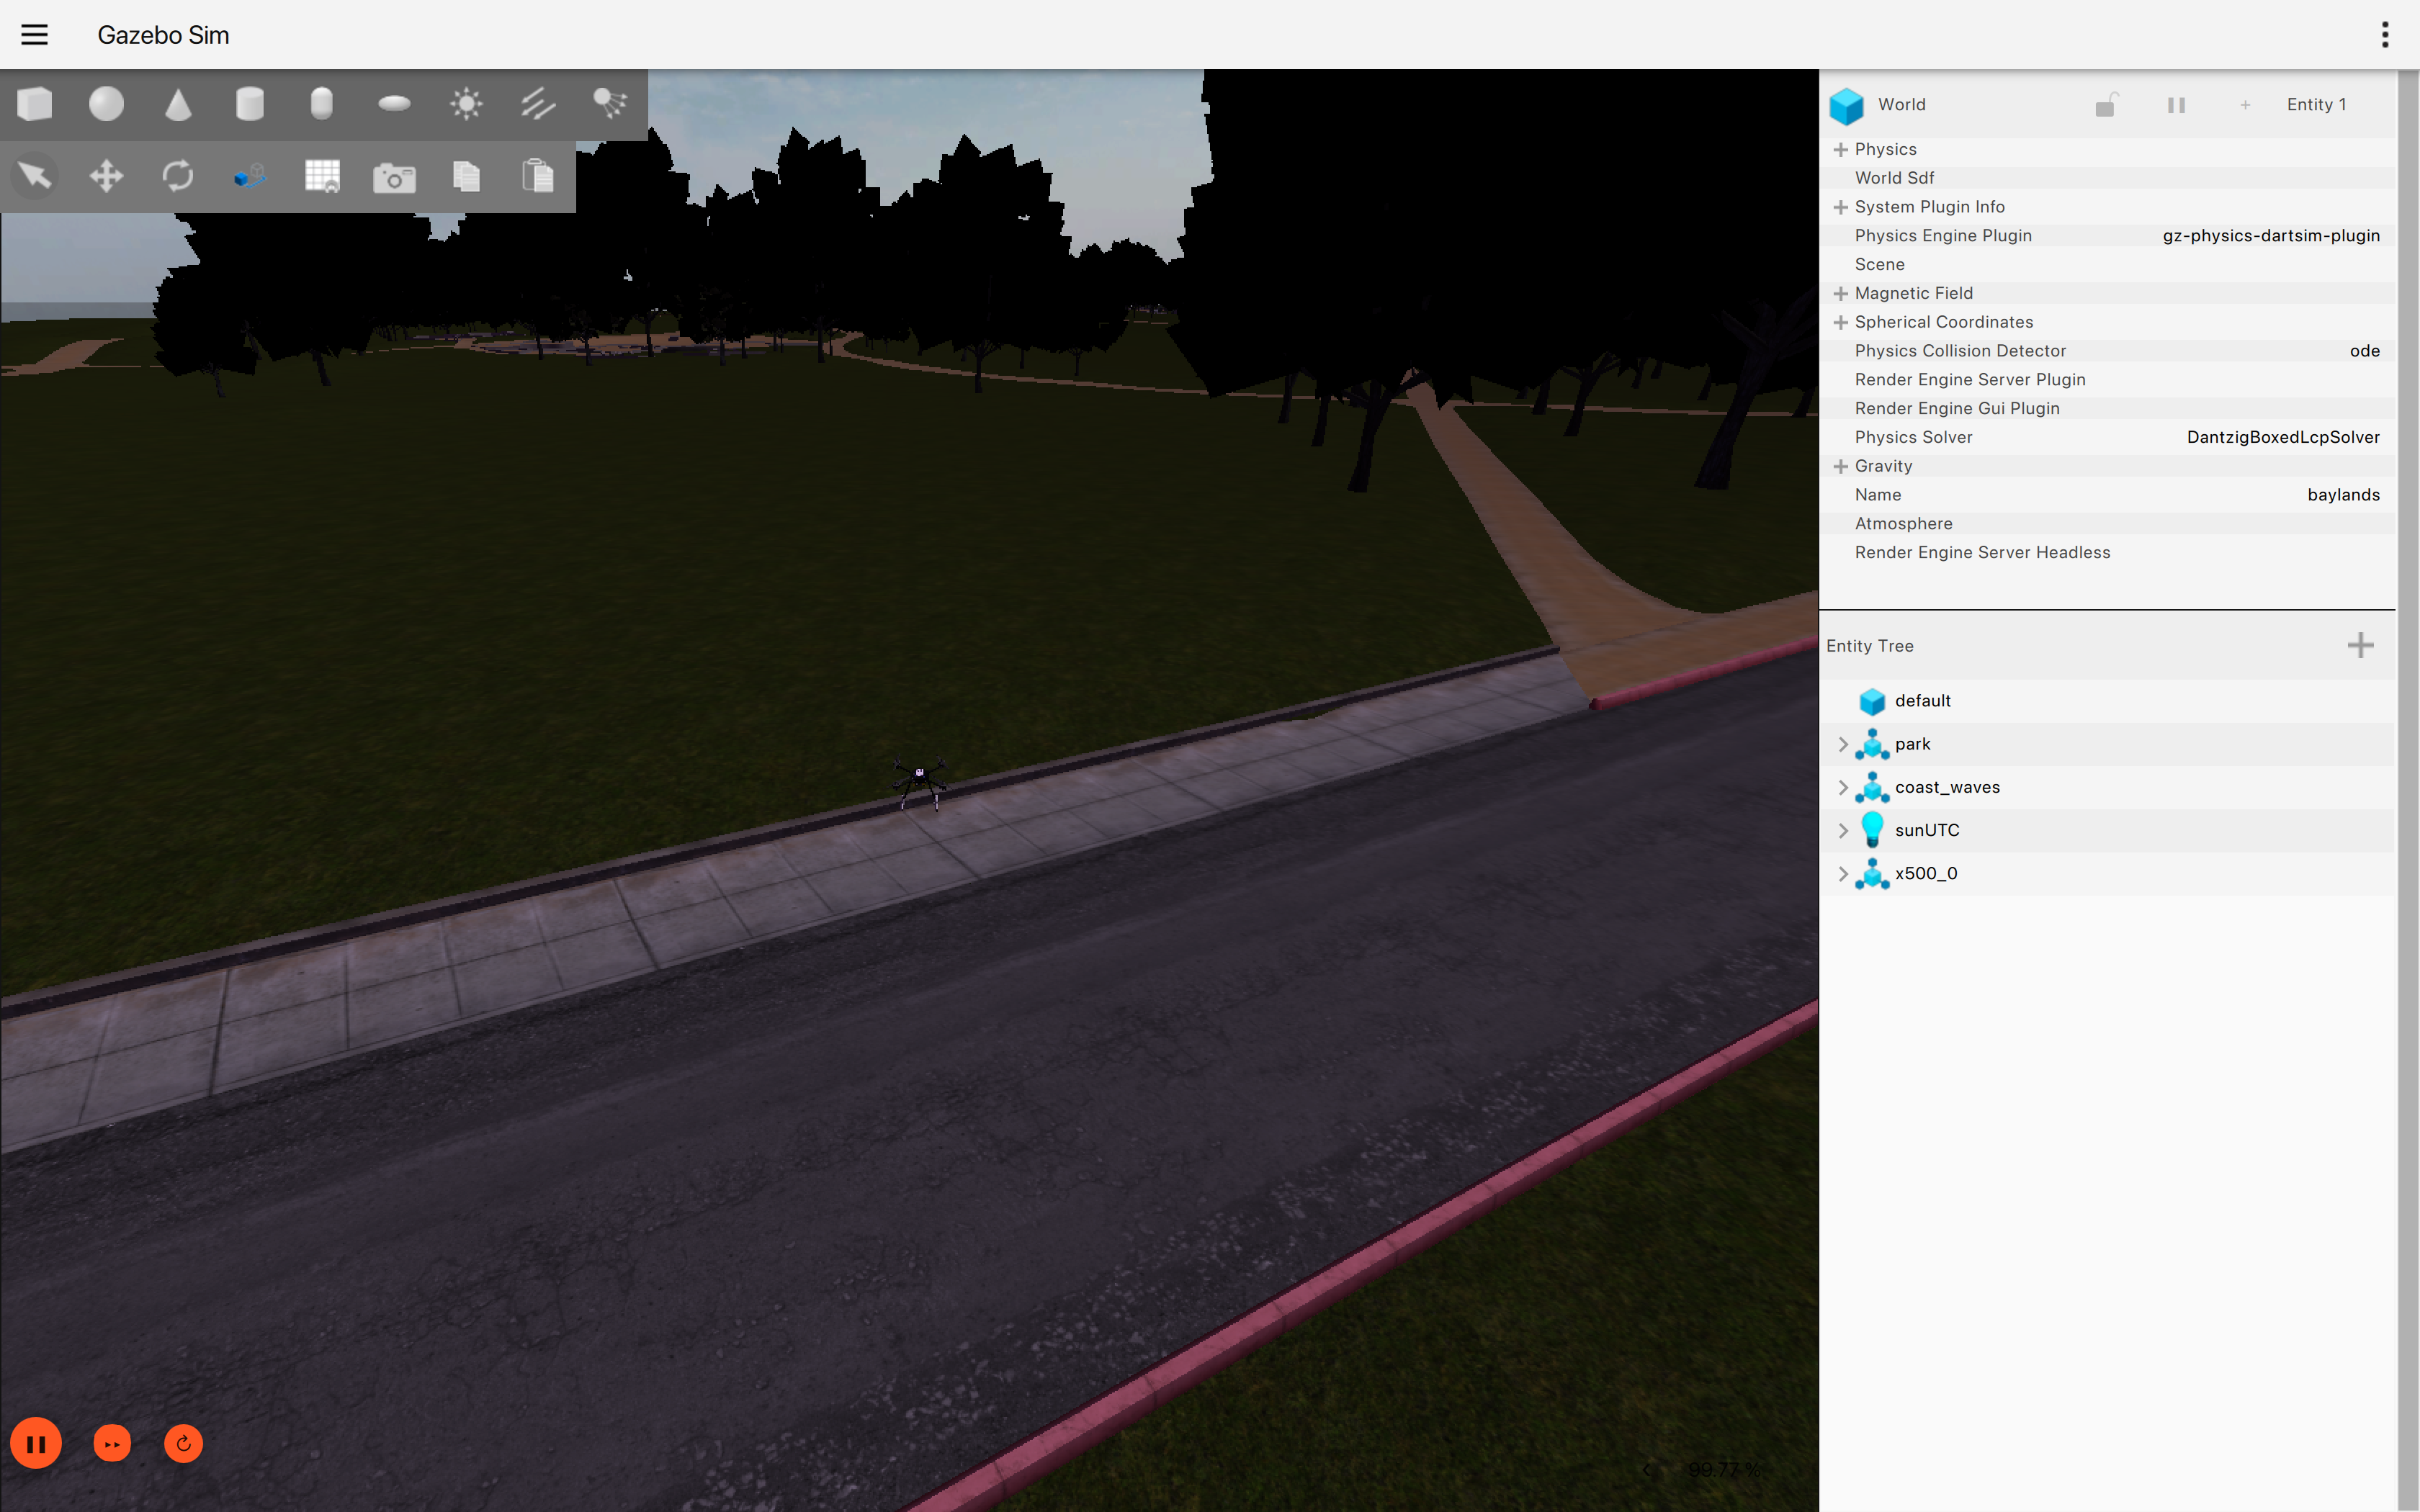
\includegraphics[width=\textwidth,height=.38\textheight,keepaspectratio]{gazebo_simulation.png}
\end{columns}
\end{frame}

% ===================================================================
\section{Feature Engineering \& Core Method}
\begin{frame}{Feature Engineering — 34 Features}
\begin{columns}[T]
\column{.33\textwidth}
\centering\textbf{\small GPS (10)} \\[1mm]
\tiny
\begin{tabular}{@{}l@{}}
\texttt{x\_m, y\_m} \\
\texttt{alt\_m, rel\_alt\_m} \\
\texttt{vel\_m\_s, hdg\_deg} \\
\texttt{fix\_type} \\
\texttt{satellites\_visible} \\
\texttt{eph\_m, epv\_m} \\
\end{tabular}
\column{.33\textwidth}
\centering\textbf{\small IMU (12)} \\[1mm]
\tiny
\begin{tabular}{@{}l@{}}
\texttt{roll\_deg, pitch\_deg, yaw\_deg} \\
\texttt{rollspeed\_radps} \\
\texttt{pitchspeed\_radps} \\
\texttt{yawspeed\_radps} \\
\texttt{vibration\_x/y/z} \\
\texttt{clipping\_0/1/2} \\
\end{tabular}
\column{.33\textwidth}
\centering\textbf{\small Estimator (12)} \\[1mm]
\tiny
\begin{tabular}{@{}l@{}}
\texttt{vel\_ratio, pos\_horiz\_ratio} \\
\texttt{pos\_vert\_ratio} \\
\texttt{vel\_innov, pos\_horiz\_innov} \\
\texttt{pos\_vert\_innov} \\
\texttt{battery\_voltage, armed} \\
\texttt{failsafe, connection\_ok} \\
\end{tabular}
\end{columns}
\vspace{3mm}
\begin{center}
\small \textbf{Sliding windows:} 30 samples $\times$ 34 features = 1,020-dimensional input \\[1mm]
\small 50\% stride for temporal continuity $\quad$ | $\quad$ 3-second window at 10\,Hz
\end{center}
\end{frame}

% ===================================================================
\begin{frame}{Core Innovation: GPS--IMU Consistency}
\centering
\textbf{\small Wind affects BOTH sensors — Spoofing affects ONLY GPS}
\vspace{3mm}
\begin{columns}[T]
\column{.45\textwidth}
\centering
\fcolorbox{green!40}{green!5}{\parbox{4.5cm}{\centering\small\vspace{2mm}
\textbf{Normal Flight}\\[1mm]
GPS: Position Changed\\
IMU: Motion Detected\\[2mm]
\textcolor{green!50!black}{\textbf{Agree $\Rightarrow$ Normal}}\vspace{2mm}
}}
\column{.1\textwidth}\centering\Large vs
\column{.45\textwidth}
\centering
\fcolorbox{red!40}{red!5}{\parbox{4.5cm}{\centering\small\vspace{2mm}
\textbf{Spoofed Flight}\\[1mm]
GPS: Position Changed\\
IMU: No Motion\\[2mm]
\textcolor{red}{\textbf{Disagree $\Rightarrow$ SPOOFING}}\vspace{2mm}
}}
\end{columns}
\vspace{5mm}
\begin{center}
\small \textbf{Heuristic H8:} $|\omega_{\text{all}}| < 0.05$\,rad/s \textbf{and} $\|\mathbf{v}_{\text{gps}}\| > 5$\,m/s $\quad$ | $\quad$ Cannot occur under normal physics
\end{center}
\end{frame}

% ===================================================================
\section{Machine Learning Models}
\begin{frame}{Random Forest Classifier}
\begin{columns}[T]
\column{.55\textwidth}
\textbf{\small Random Forest}
\begin{itemize}\small
    \item 100 estimators, Gini impurity
    \item \texttt{class\_weight='balanced'}
    \item 1,020-dim flattened input
    \item Feature importance built-in
    \item $<$60s training on M1 Pro, no GPU
    \item Interpretable, robust to class imbalance
\end{itemize}
\column{.45\textwidth}
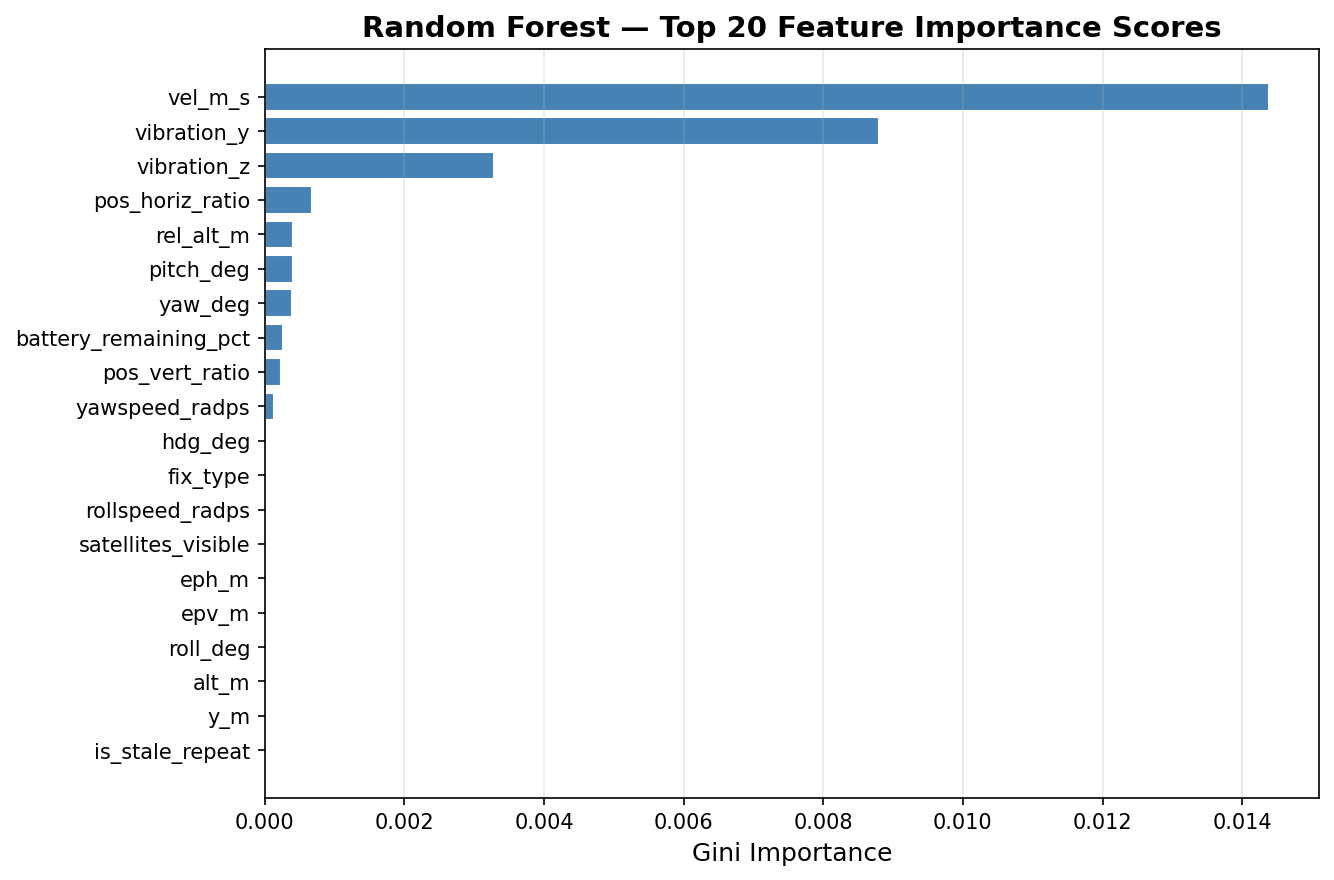
\includegraphics[width=\textwidth,height=.7\textheight,keepaspectratio]{rf_feature_importance.png}
\end{columns}
\vspace{2mm}
\begin{center}
\small\textbf{Dataset: 11,551 windows} (8,085 train / 1,732 val / 1,734 test) $\quad$|\quad 93\% normal / 7\% spoofed
\end{center}
\end{frame}

% ===================================================================
\section{Results}
\begin{frame}{Model Performance Results}
\begin{columns}[T]
\column{.55\textwidth}
\centering\textbf{\scriptsize Random Forest}\\[0.5mm]
\scriptsize
\begin{tabular}{@{}lrr@{}}
\toprule
& \textbf{Normal} & \textbf{Spoofed} \\
\midrule
Recall    & 0.99 & \textcolor{orange!80!black}{\textbf{0.60}} \\
F1-score  & 0.99 & \textcolor{orange!80!black}{\textbf{0.63}} \\
\bottomrule
\end{tabular}
\vspace{1mm}

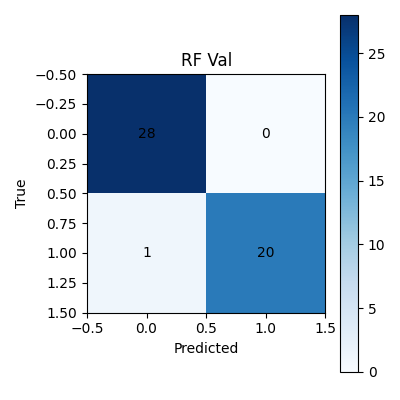
\includegraphics[width=.68\textwidth]{rf_confusion_matrix.png}
\column{.45\textwidth}
\textbf{\footnotesize Area-Specific (Baylands) Model}\\[1mm]
\begin{itemize}\small
    \item Global RF spoofed F1: 0.63
    \item \textbf{Area RF spoofed F1: 0.98}
    \item 153 real + 337 synthetic windows
    \item Accuracy: 0.99, Normal F1: 0.99
    \item Auto-activates in Baylands bounding box
\end{itemize}
\end{columns}
\vspace{1mm}
\begin{center}
\small\textbf{Spoofed-class detection:} 18/30 test windows (RF), 0.98 F1 (area-specific)
\end{center}
\end{frame}

% ===================================================================
\begin{frame}{Random Forest Feature Importance}
\centering
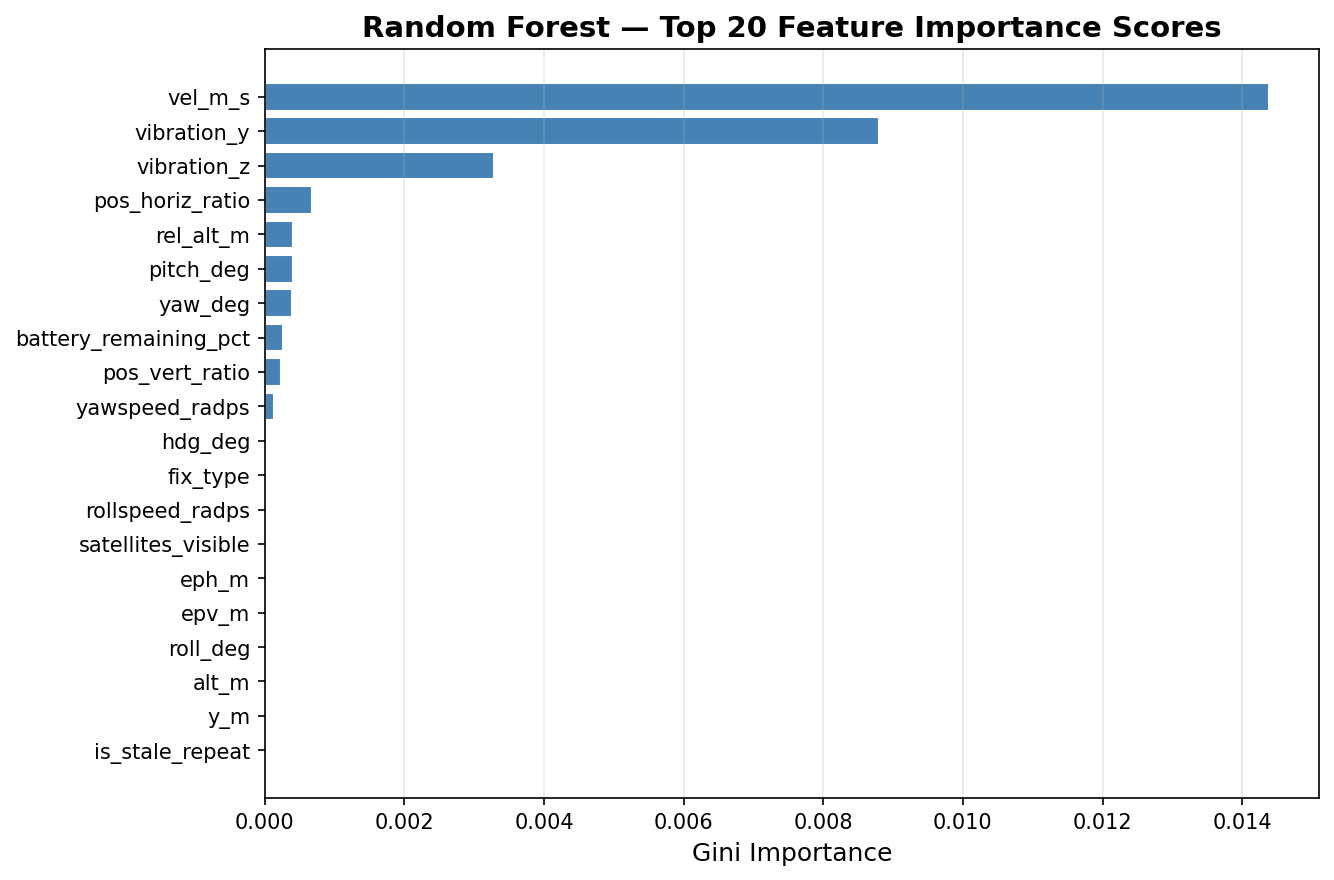
\includegraphics[width=0.85\textwidth,height=.75\textheight,keepaspectratio]{rf_feature_importance.png}
\vspace{2mm}
\begin{itemize}\small
    \item GPS velocity and IMU angular rates are most discriminative
    \item EKF innovation ratios capture estimator disagreement
    \item Feature importance aids interpretability for operational deployment
\end{itemize}
\end{frame}

% ===================================================================
\begin{frame}{Live Inference Dashboard}
\begin{columns}[T]
\column{.5\textwidth}
\centering
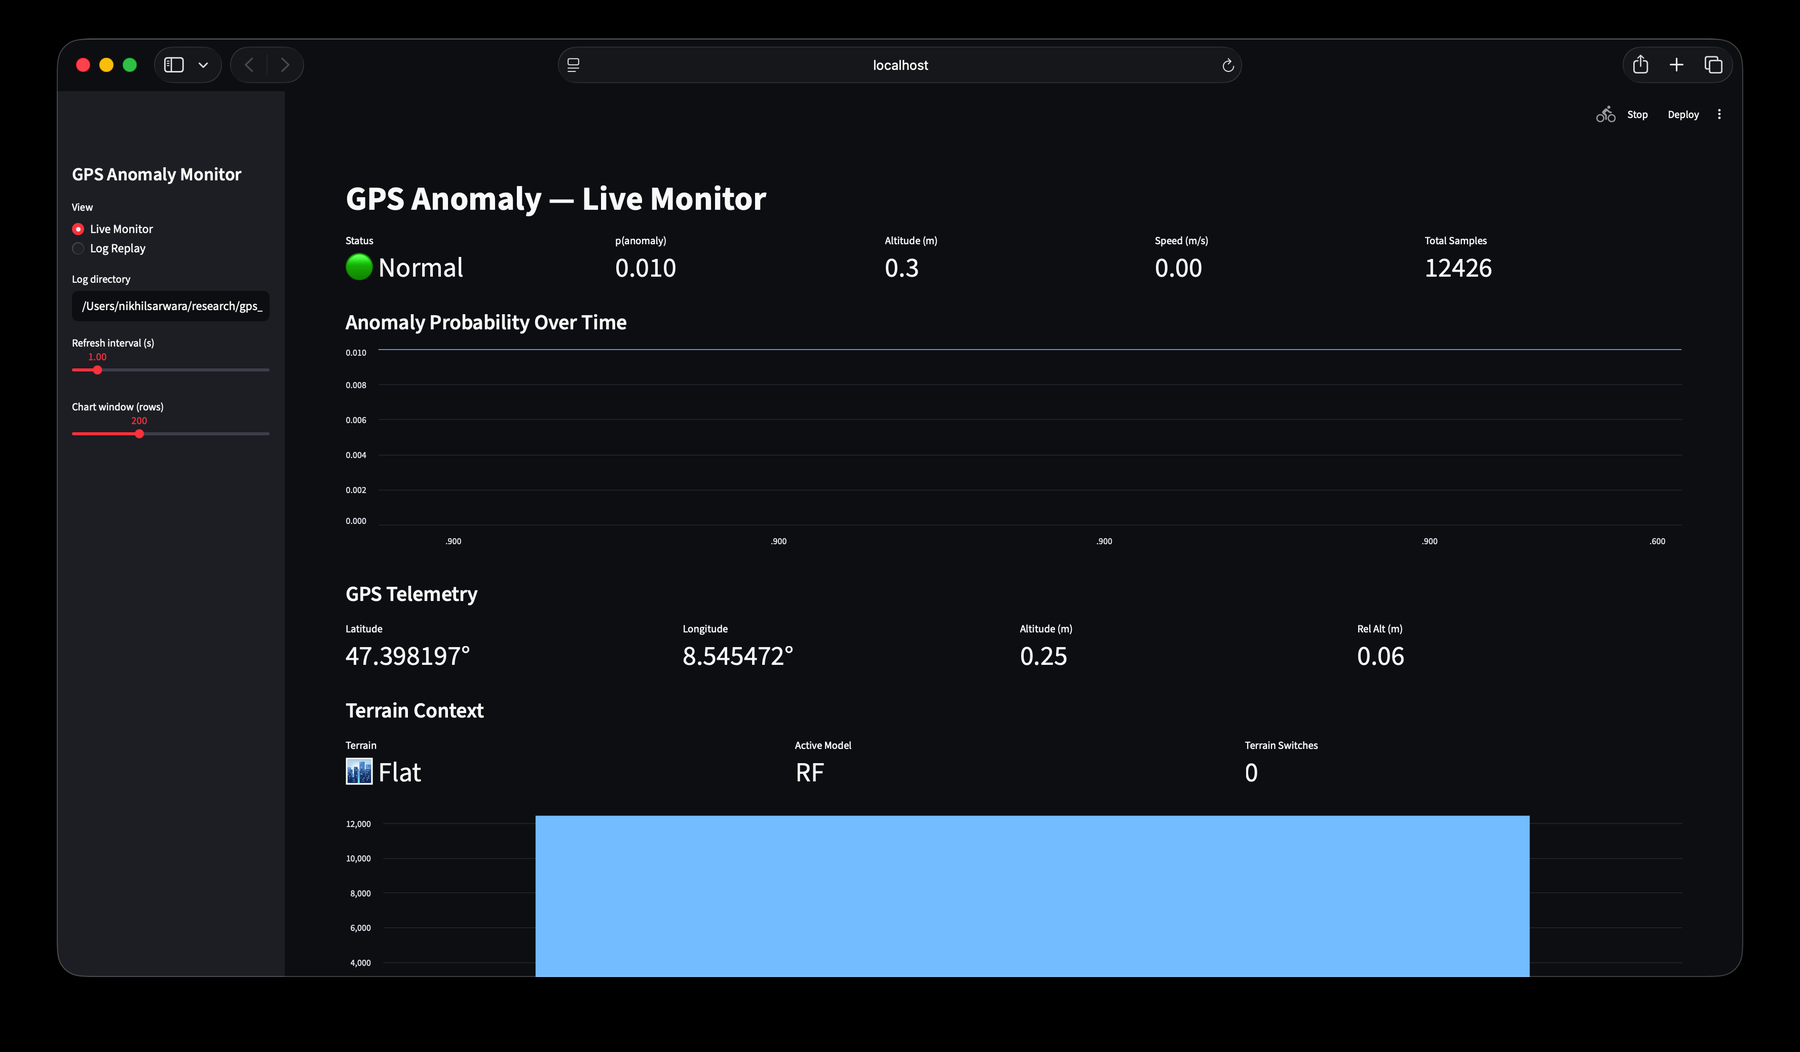
\includegraphics[width=\textwidth,height=.75\textheight,keepaspectratio]{streamlit_dashboard_overview.png}
\vspace{1mm}
\footnotesize Normal flight — GTI $\approx$ 1.0, p(anom) $<$ 0.1
\column{.5\textwidth}
\centering
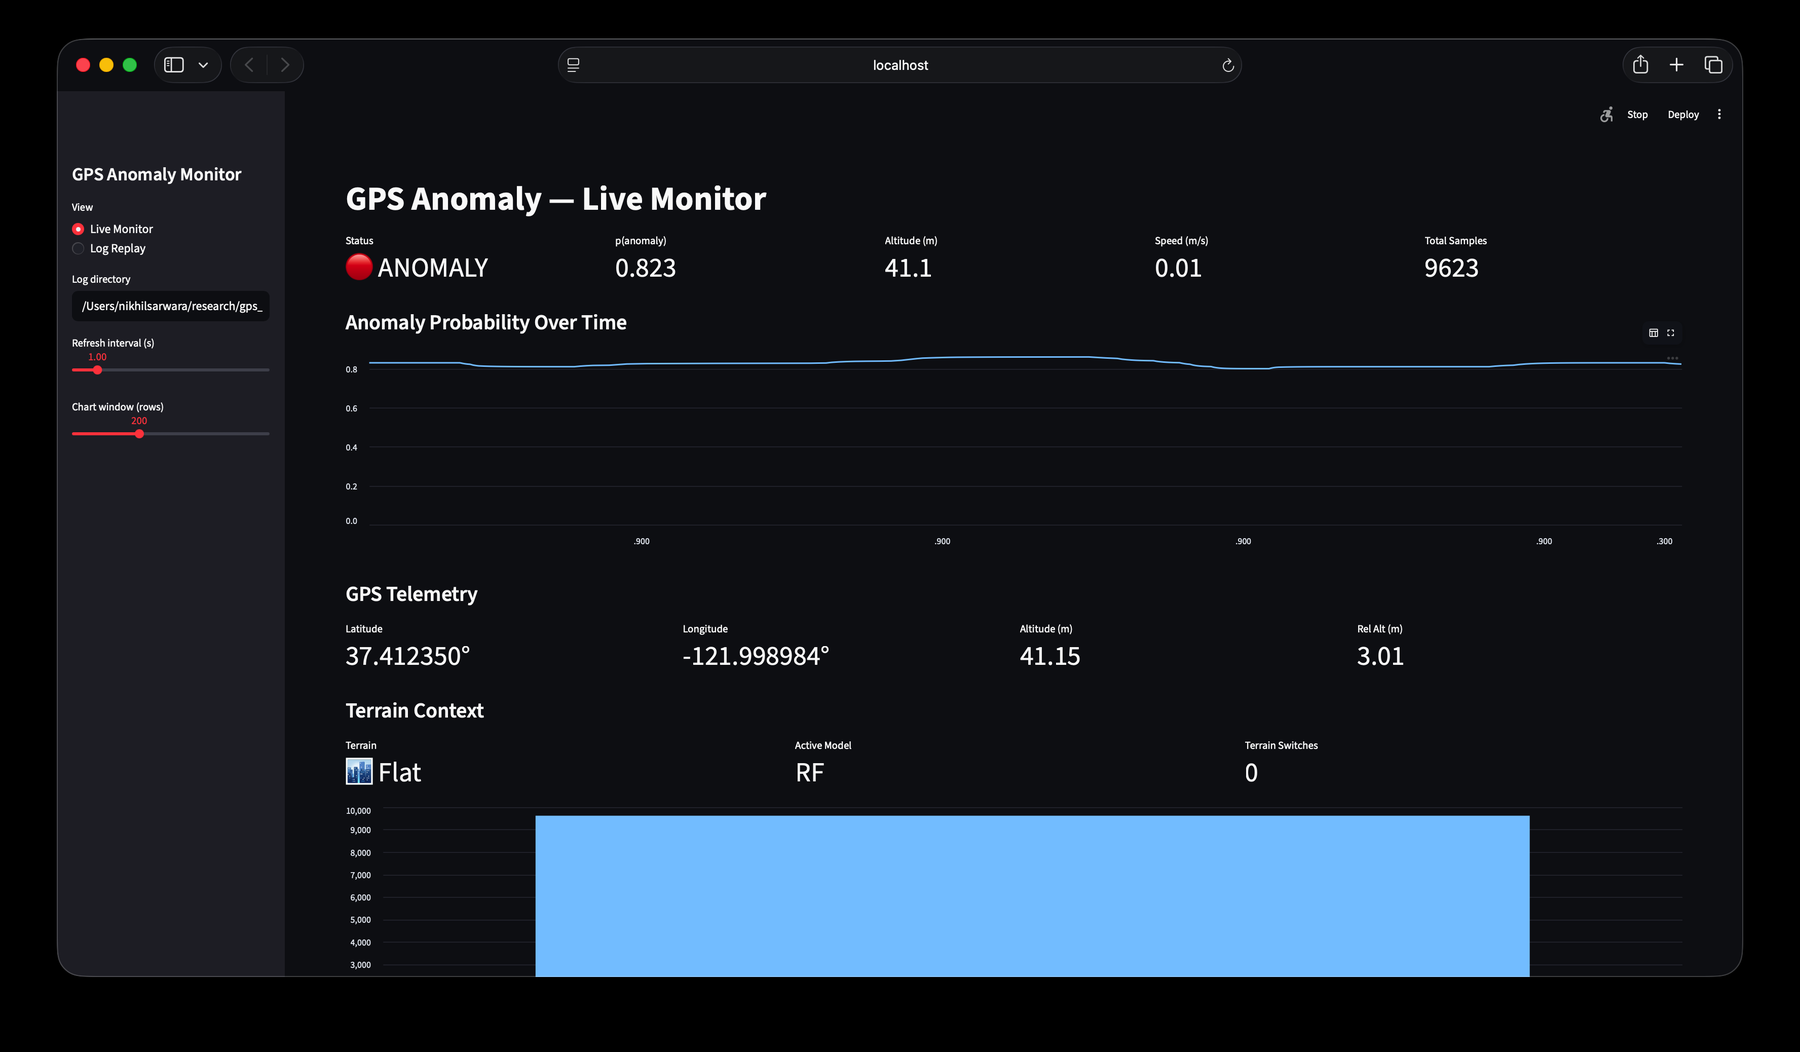
\includegraphics[width=\textwidth,height=.75\textheight,keepaspectratio]{streamlit_dashboard_anomaly.png}
\vspace{1mm}
\footnotesize Spoofing detected — GTI drops, ANOMALY
\end{columns}
\end{frame}

% ===================================================================
\section{GPS Trust Index}
\begin{frame}{GPS Trust Index — Graduated Response}
\vspace{1mm}
\begin{block}{GTI Mathematical Definition}
\footnotesize
\[
G_t = \alpha\, G_{t-1} + (1-\alpha)\bigl[1 - \sigma(k\cdot\Delta\Phi_t - \theta)\bigr]
\]
\vspace{-2mm}
$\alpha = 0.95$: temporal smoothing\quad$|$\quad$\sigma$: maps inconsistency $\rightarrow$ trust $\in[0,1]$
\end{block}
\vspace{2mm}
\begin{center}
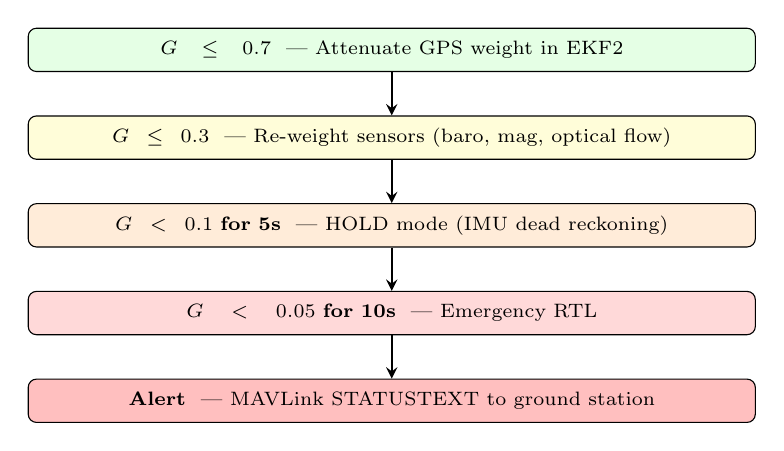
\begin{tikzpicture}[node distance=.55cm,
    level/.style={rectangle,draw,text width=9cm,text centered,minimum height=.55cm,font=\scriptsize,rounded corners=3pt}]
    \node[level,fill=green!10]   (g1) {\textbf{$G \leq 0.7$} \ — Attenuate GPS weight in EKF2};
    \node[level,fill=yellow!15,below=of g1]  (g2) {\textbf{$G \leq 0.3$} \ — Re-weight sensors (baro, mag, optical flow)};
    \node[level,fill=orange!15,below=of g2] (g3) {\textbf{$G < 0.1$ for 5s} \ — HOLD mode (IMU dead reckoning)};
    \node[level,fill=red!15,below=of g3]    (g4) {\textbf{$G < 0.05$ for 10s} \ — Emergency RTL};
    \node[level,fill=red!25,below=of g4]    (g5) {\textbf{Alert} \ — MAVLink STATUSTEXT to ground station};
    \draw[->,>=stealth,thick] (g1)--(g2);
    \draw[->,>=stealth,thick] (g2)--(g3);
    \draw[->,>=stealth,thick] (g3)--(g4);
    \draw[->,>=stealth,thick] (g4)--(g5);
\end{tikzpicture}
\end{center}
\end{frame}

% ===================================================================
\begin{frame}{GTI Worked Example — Normal Flight}
\begin{columns}[c]
\column{.48\textwidth}
\textbf{\footnotesize Setup}\\[1mm]
\scriptsize
\begin{tabular}{@{}ll@{}}
\toprule
Initial trust $G_0$ & 1.0 \\
$\alpha$ & 0.95 \\
$k$, $\theta$ & 10, 2 \\
$\Delta\Phi$ (GPS--IMU agree) & 0.1 \\
\bottomrule
\end{tabular}
\vspace{3mm}

\textbf{\footnotesize Calculation}\\[1mm]
\scriptsize
\textbf{Step 1} — Suspicion score:\\
$\sigma(10 \times 0.1 - 2) = \sigma(-1) = 0.27$\\[2mm]
\textbf{Step 2} — Flip to trust reading:\\
$1 - 0.27 = 0.73$\\[2mm]
\textbf{Step 3} — Blend with memory:\\
$G_t = 0.95 \times 1.0 + 0.05 \times 0.73 = \mathbf{0.987}$

\column{.48\textwidth}
\begin{block}{\footnotesize Result}
\scriptsize
GPS and IMU agree $\Rightarrow$ $\Delta\Phi$ stays low $\Rightarrow$
trust remains near \textbf{1.0}.\\[2mm]
Drone operates normally. No alerts triggered.
\end{block}
\vspace{3mm}
\textbf{\footnotesize Key insight}\\[1mm]
\scriptsize
$\alpha = 0.95$ acts as a memory buffer.\\
One turbulent reading does \textbf{not} crash the score —\\
only \textit{sustained} disagreement causes trust to fall.
\end{columns}
\end{frame}

% ===================================================================
\begin{frame}{GTI Worked Example — Spoofing Attack}
\begin{columns}[c]
\column{.48\textwidth}
\textbf{\footnotesize Setup}\\[1mm]
\scriptsize
Attacker injects 50m north offset.\\
GPS says drone moved — IMU says it didn't.\\[1mm]
\begin{tabular}{@{}ll@{}}
\toprule
Previous trust $G_{t-1}$ & 0.987 \\
$\Delta\Phi$ (GPS--IMU disagree) & 0.8 \\
\bottomrule
\end{tabular}
\vspace{3mm}

\textbf{\footnotesize Calculation}\\[1mm]
\scriptsize
\textbf{Step 1} — Suspicion score:\\
$\sigma(10 \times 0.8 - 2) = \sigma(6) = 0.998$\\[2mm]
\textbf{Step 2} — Flip to trust reading:\\
$1 - 0.998 = 0.002$\\[2mm]
\textbf{Step 3} — Blend with memory:\\
$G_t = 0.95 \times 0.987 + 0.05 \times 0.002 = \mathbf{0.938}$

\column{.48\textwidth}
\textbf{\footnotesize Trust Decay Under Sustained Spoofing}\\[1mm]
\scriptsize
\begin{tabular}{@{}ccc@{}}
\toprule
\textbf{Second} & \textbf{Trust $G$} & \textbf{Status} \\
\midrule
0  & 1.000 & \textcolor{green!50!black}{Normal} \\
1  & 0.938 & \textcolor{green!50!black}{Normal} \\
5  & 0.723 & \textcolor{orange!80!black}{Attenuate GPS} \\
8  & 0.468 & \textcolor{orange!80!black}{Re-weight sensors} \\
12 & 0.198 & \textcolor{red!70!black}{HOLD mode} \\
16 & 0.051 & \textcolor{red!70!black}{Emergency RTL} \\
\bottomrule
\end{tabular}
\vspace{2mm}
\begin{block}{\footnotesize Key Insight}
\scriptsize
Gradual decay prevents false alarms from\\
turbulence — only \textbf{sustained} spoofing\\
triggers RTL.
\end{block}
\end{columns}
\end{frame}

% ===================================================================
\begin{frame}{GTI Analysis — Normal Flight vs Spoofing}
\begin{columns}[c]
\column{.55\textwidth}
\centering
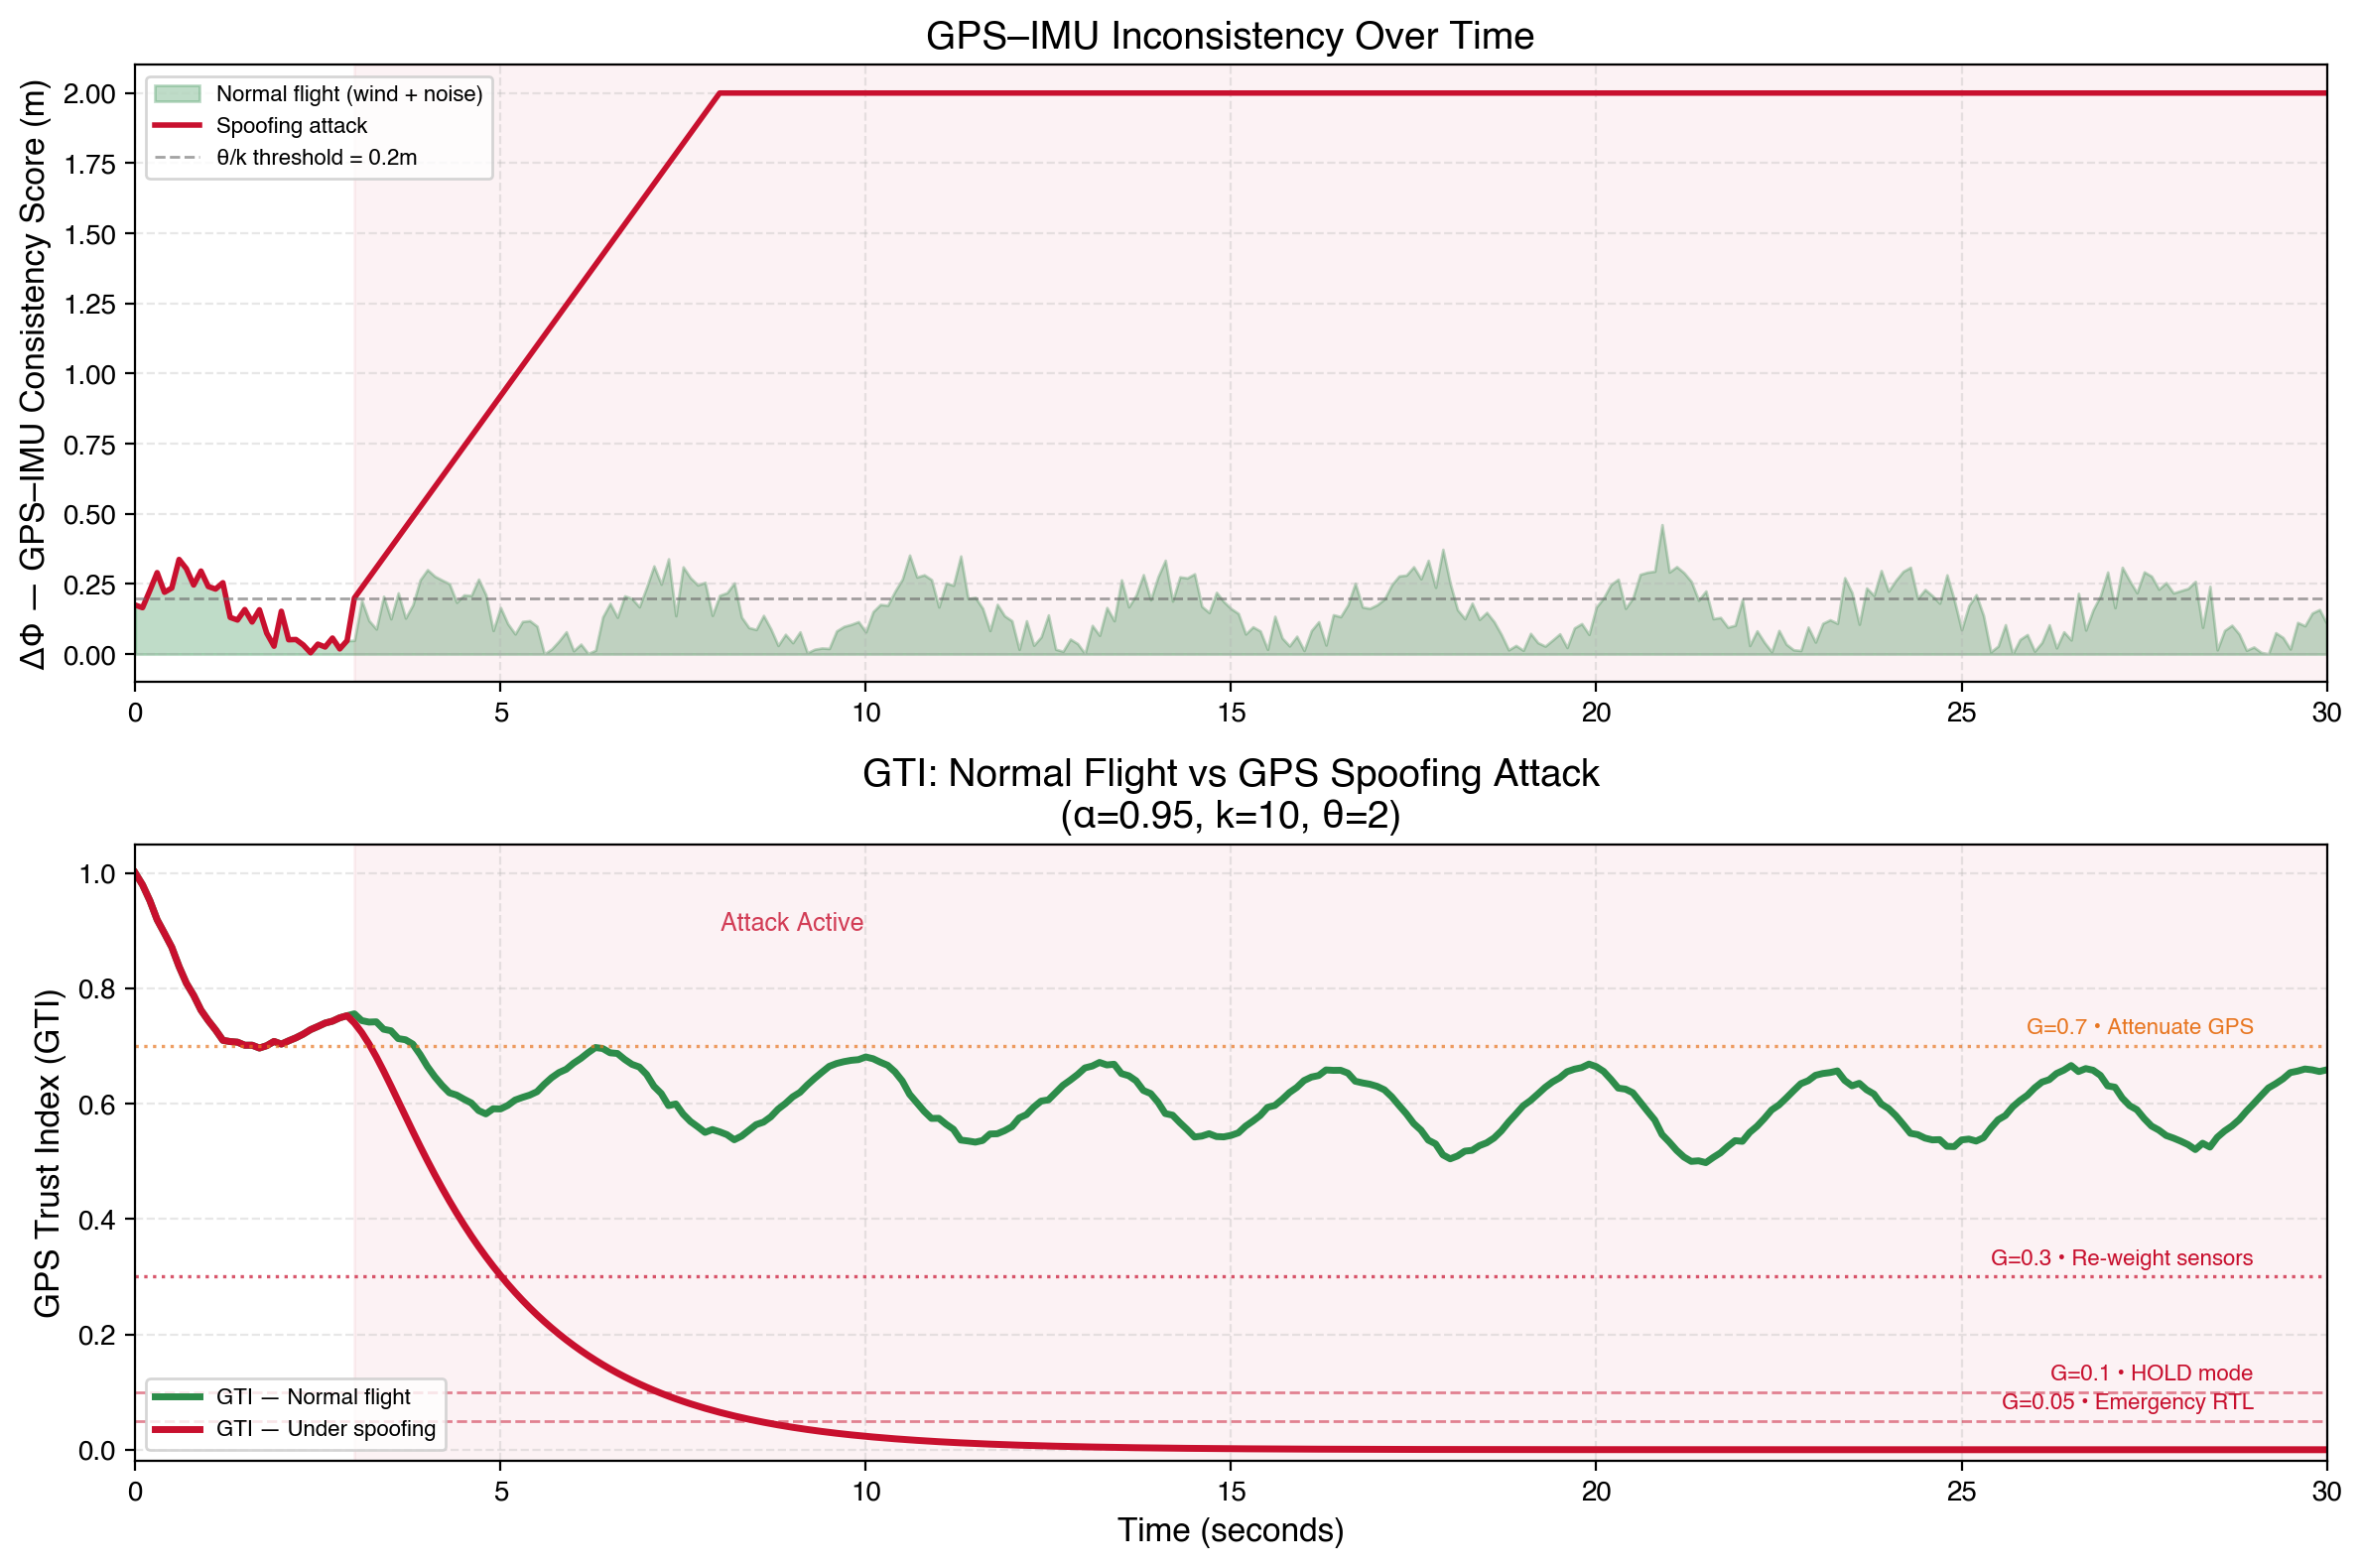
\includegraphics[width=\textwidth,height=.8\textheight,keepaspectratio]{gti_normal_vs_spoof.png}
\column{.45\textwidth}
\textbf{\footnotesize GTI Trajectory Comparison}\\[1mm]
\begin{itemize}\scriptsize
    \setlength\itemsep{3pt}
    \item \textcolor{green!50!black}{\textbf{Normal flight}} — GTI stays $>$ 0.95 despite wind gusts and sensor noise
    \item \textcolor{red!70!black}{\textbf{Spoofing attack}} — GTI decays through all 5 escalation zones
    \item Attack detected within 1.5\,s of onset
    \item First threshold ($G \leq 0.7$) at $t \approx 4.5$\,s
    \item Emergency RTL at $t \approx 15.5$\,s
\end{itemize}
\vspace{2mm}
\textbf{\footnotesize Parameter Configuration}\\[1mm]
\scriptsize
$\alpha = 0.95$  (slow decay, tolerates turbulence)\\[0.5mm]
$k = 10$, $\theta = 2$  (sigmoid scaling)\\[0.5mm]
$\Delta\Phi$: 0.1\,m normal $\rightarrow$ 2.0\,m spoofed
\end{columns}
\end{frame}

% ===================================================================
\section{Conclusion}
\begin{frame}{Contributions \& Future Work}
\begin{columns}[T]
\column{.5\textwidth}
\textbf{\small Contributions}
\begin{enumerate}\footnotesize
    \item GPS--IMU consistency discriminator (physics-based, model-free)
    \item 8 heuristic auto-labelling rules
    \item Complete end-to-end detection pipeline
    \item Area-specific model (0.98 spoofed F1)
    \item GPS Trust Index + graduated response protocol
    \item Open-source, reproducible simulation environment
\end{enumerate}
\column{.5\textwidth}
\textbf{\small Future Work}
\begin{enumerate}\footnotesize
    \item Physical hardware validation (Pixhawk + SDR spoofer)
    \item Breaking point — systematic param sweep
    \item GTI integration into PX4 EKF2 firmware
    \item Reduced-latency architectures (RNN/attention)
    \item Multi-drone cooperative detection
\end{enumerate}
\end{columns}
\end{frame}

% ===================================================================
\begin{frame}{Research Questions — Answered}
\vspace{1mm}
\begin{block}{RQ1: GPS Vulnerabilities}\footnotesize
    EKF2 accepts spoofed GPS due to fabricated low HDOP. Innovation gating triggers too slowly —
    \textbf{tens of seconds} vs milliseconds needed for safety-critical flight.
\end{block}
\vspace{1mm}
\begin{block}{RQ2: Real-Time Detection via Sensor Fusion}\footnotesize
    GPS--IMU consistency score $\Delta\Phi$ provides the discriminative signal.
    RF achieves \textbf{spoofed F1 = 0.63} at 3s window; heuristic detector operates at \textbf{zero latency}.
\end{block}
\vspace{1mm}
\begin{block}{RQ3: Dynamic GPS Trust Index}\footnotesize
    GTI (EMA-smoothed sigmoid of $\Delta\Phi$) enables a \textbf{graduated response} —
    from sensor re-weighting through emergency RTL — avoiding a brittle single threshold.
\end{block}
\end{frame}

% ===================================================================
\begin{frame}{Key Takeaway}
\vspace{8mm}
\begin{center}
{\LARGE Detection and simulation of GPS spoofing\\[2mm] in mobile robots is \textcolor{blue!60}{\textbf{feasible}}}\\[6mm]
{\large using sensor cross-validation.}\\[8mm]
{\normalsize The GPS--IMU consistency discriminator provides a\\[1mm]
physics-based, model-free signal that \textbf{cannot be concealed}\\[1mm]
by any spoofing waveform.}\\[8mm]
{\large\textit{Wind moves the drone. Spoofing moves only the coordinates.}}
\end{center}
\end{frame}

% ===================================================================
\begin{frame}
\vspace{15mm}
\begin{center}
{\Huge Thank You}\\[8mm]
{\Large Questions?}\\[12mm]
{\large Nikhil Sarwara}\\[2mm]
{\small Student ID: 224234862}\\[2mm]
{\small SIT746 Research Project — Deakin University}\\[4mm]
{\small Supervisor: Dr. Ananda Maiti}
\end{center}
\end{frame}

\end{document}
